\documentclass[12pt,letterpaper]{article}
\usepackage[utf8]{inputenc}
\usepackage{tikz}
\usepackage[hidelinks]{hyperref}
\usepackage{graphicx}
\author{Curso de \LaTeX}
\title{Ejemplo de un árbol filogenético construido desde \LaTeX}
\begin{document}
\maketitle
Existen varias herramientas de \LaTeX\ para construir gráficos de árboles, y una que resulta especialmente útil para los árboles filogenéticos se encuentra en el paquete  \texttt{tikz}, a través del comando \texttt{child}.

Ejemplo de un árbol filogenético enraizado:

\begin{center}
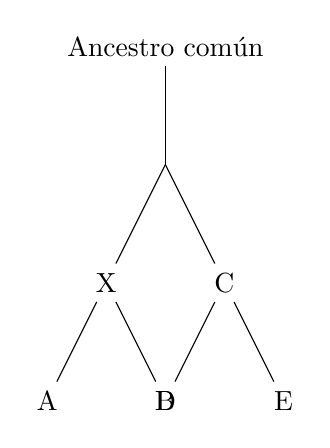
\begin{tikzpicture}
  \node {Ancestro común}
    child {
		child {
			node {X}
			child { node {A} }
      		child { node {B} }
    	}
    	child { node {C}
    		child{ node {D}}
    		child{ node {E}}}
    };
\end{tikzpicture}
\end{center}

Podemos modificar el diseño de las ramas del árbol con las distintas opciones que nos ofrece esta biblioteca, por ejemplo el largo de las ramas y su separación:

\begin{center}
\begin{tikzpicture}[level distance=60pt] %distancia entre cada nivel del árbol
  \node {Ancestro común}
    child {
		child {
			child { node {A} }
      		child { node {B} }
    	}
    	child { node {C}}
    };
\end{tikzpicture}

\begin{tikzpicture}[sibling distance=72pt] %distancia entre los hijos
  \node {Ancestro común}
    child {
		child {
			child { node {A} }
      		child { node {B} }
    	}
    	child { node {C}}
    };
\end{tikzpicture}
\end{center}

También podemos hacer que el árbol crezca en diferentes direcciones:

\begin{center}
\begin{tikzpicture}[grow=right, sibling distance=72pt]
\node {}
child {
	child {
		child { node {Selangileas} }
   		child { node {Isoetes} }
   	}
   	child { node {Licopodios}}
};
\end{tikzpicture}
\end{center}

Cuando el árbol crece más, es necesario ampliar la distancia entre sus ramas, para que estas no se solapen. Para conseguirlo, podemos aplicar una distancia diferente entre las ramas a cada uno de los niveles del árbol:

\begin{center}
\begin{tikzpicture}[grow=right, level distance=2cm,
  level 1/.style={sibling distance=1cm},
  level 2/.style={sibling distance=3cm},
  level 3/.style={sibling distance=1.5cm}]
\node {Ancestro común}
child {
	child {
		child {
			child { node {Selangileas} }
	   		child { node {Isoetes} }
	   	}
	   	child { node {Licopodios}}
	}
	child {
		child { node {Plantas con flores} }
		child { node {Helechos} }
	}
};
\end{tikzpicture} %Como vemos, es posible definir la distancia en cada uno de los niveles del árbol (3 en este ejemplo) con la opción level <no>. 
\end{center}

Si el primer nivel del árbol contendrá solo a la raíz del mismo, podemos omitir definir la distancia de las ramas en este nivel y comenzar a hacerlo a partir del segundo nivel, por ejemplo para un árbol de 5 niveles:

\begin{tikzpicture}[level 2/.style={sibling distance=4cm},
  level 3/.style={sibling distance=2cm},
  level 4/.style={sibling distance=1cm},
  level 5/.style={sibling distance=0.75cm},
  level distance=1cm]
\node {Ancestro común}
child {
	child {
    	child {
			child { node {A} }
    		child { node {B} }
    	}
		child {
			child {
				child { node {D} }
				child { node {E} }
			}
			child { node {F} }
		}
	}
	child {
		child {
			child { node {G} }
			child { node {H} }
			child { node {I} }
		}
		child { node {J} }
	}
	child {
		child {
			child {
				child { node {J} }
				child { node {K} }
			}
			child { node {M} }
		}
		child {
			child { node{N} }
		}
		child { node{O} }
	}
};   
\end{tikzpicture}


Un árbol filogenético representado con un cladograma, requeriría de un cambio adicional para conseguir que las ramas mostraran un ángulo recto:

\begin{tikzpicture} [level 2/.style={sibling distance=4cm},
  level 3/.style={sibling distance=2cm},
  level 4/.style={sibling distance=1cm},
  grow=right, 
  edge from parent path={(\tikzparentnode.east) |- (\tikzchildnode.west)}, level distance=2.5cm]
\node {}
child {      
	child {
	   	child { node {
\includegraphics[width=24px]{img/bee.png}} }
    	child {
        	child { node {
\includegraphics[width=24px]{img/butterfly.png}} }
	        child { node {
\includegraphics[width=24px]{img/fly.png}} }
	    }
      }
	child { node {
\includegraphics{img/bug.png}} }
};   
\end{tikzpicture} %Utilizamos la opción [edge from parent path] para modificar la forma en la que se dibujan las ramas desde la rama padre hacia sus ramas hijas.

Nota: el cladograma anterior muestra la relación entre varios grupos de insectos.

Si quisiéramos poner al mismo nivel a todas las hojas del árbol, podemos modificar su distancia en las opciones de cada comando \texttt{child}:

\begin{tikzpicture} [level 2/.style={sibling distance=4cm},
  level 3/.style={sibling distance=2cm},
  level 4/.style={sibling distance=1cm},
  grow=right, 
  edge from parent path={(\tikzparentnode.east) |- (\tikzchildnode.west)}, level distance=2.5cm]
\node {}
child {      
	child {
	   	child[level distance=5cm] { node {
\includegraphics[width=24px]{img/bee.png}} }
    	child {
        	child { node {
\includegraphics[width=24px]{img/butterfly.png}} }
	        child { node {
\includegraphics[width=24px]{img/fly.png}} }
	    }
      }
	child[level distance=7.5cm] { node {
\includegraphics{img/bug.png}} }
};   
\end{tikzpicture}

Para conocer el resto de las opciones para árboles del paquete \texttt{tikz} y ver ejemplos más avanzados, puedes consultar su documentación completa en la siguiente dirección: \url{http://www.sfu.ca/~haiyunc/notes/Game\_Trees\_with\_TikZ.pdf}

\end{document}